\chapter{Eulerian and Hamiltonian problems}
\section*{One trip, every road}
An Euler trail uses every edge exactly once. It may begin and end at different vertices. An Euler circuit is a closed Euler trail. A graph with at least one edge is \emph{Eulerian} if it has an Euler circuit; isolated vertices are allowed. The distinction between covering edges and covering vertices is fundamental.

\begin{theorem}[\Core{} Euler criterion]
A connected graph with at least one edge has an Euler circuit if and only if every vertex has even degree. It has an open Euler trail if and only if exactly two vertices have odd degree.
\end{theorem}
\begin{figure}[htbp]
\centering
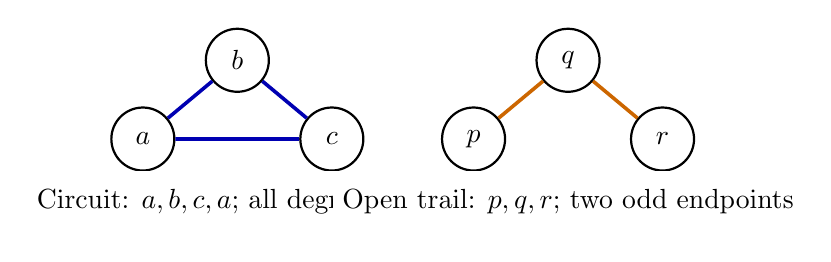
\begin{tikzpicture}[thick,every node/.style={circle,draw,fill=white,minimum size=8mm}]
\node (a) at (0,0) {$a$}; \node (b) at (1.2,1) {$b$}; \node (c) at (2.4,0) {$c$};
\draw[blue!70!black,line width=1.3pt] (a)--(b)--(c)--(a);
\node[draw=none,rectangle] at (1.2,-0.8) {Circuit: $a,b,c,a$; all degrees even};
\node (p) at (4.2,0) {$p$}; \node (q) at (5.4,1) {$q$}; \node (r) at (6.6,0) {$r$};
\draw[orange!80!black,line width=1.3pt] (p)--(q)--(r);
\node[draw=none,rectangle] at (5.4,-0.8) {Open trail: $p,q,r$; two odd endpoints};
\end{tikzpicture}
\caption{Euler circuits have no odd-degree vertices; open Euler trails have exactly two.}
\end{figure}
\begin{proof}
In any trail, each time the trail enters a vertex it must leave along a different unused edge. In a closed trail, these arrivals and departures pair up at every vertex, so all degrees are even. In an open trail, the start has one extra departure and the end one extra arrival, so precisely those two vertices have odd degree.

For sufficiency in the all-even case, start at any vertex and follow unused edges until no continuation is possible. At any vertex other than the start, arriving uses one edge, so an unused exit remains whenever the walk has not exhausted that vertex's incident edges. Thus the walk closes at its start. If unused edges remain, connectedness ensures some vertex on the closed walk is incident with an unused edge. Starting there, construct another closed trail of unused edges and splice it into the first. Repeat; finiteness ensures termination with an Euler circuit.

If exactly two vertices are odd, add one extra edge between them. The augmented graph is connected and all-even, so it has an Euler circuit. Removing the added edge leaves an Euler trail with the two odd vertices as endpoints. The necessary parity argument shows no other cases are possible.
\end{proof}

The connectedness condition matters: two disjoint cycles have only even degrees but no single walk can cover both. Isolated vertices can be disregarded if the graph has edges, but all non-isolated vertices must lie in one component.

A practical construction is Hierholzer's method: follow unused edges until returning to the start, then splice in further closed trails wherever unused edges remain. Fleury's rule (avoid a bridge unless forced) is another hand method, though it is less efficient.

A \emph{Hamiltonian path} is a path that visits every vertex exactly once. A \emph{Hamiltonian cycle} visits every vertex exactly once before returning to its start, and a graph containing one is called a \emph{Hamiltonian graph}. Unlike Euler circuits, there is no simple degree-parity test that characterises Hamiltonian graphs. A necessary condition is that every vertex have degree at least 2, but this is not sufficient: two triangles joined by a single bridge have minimum degree (the smallest vertex degree) 2 and no Hamiltonian cycle.

\begin{figure}[htbp]
\centering
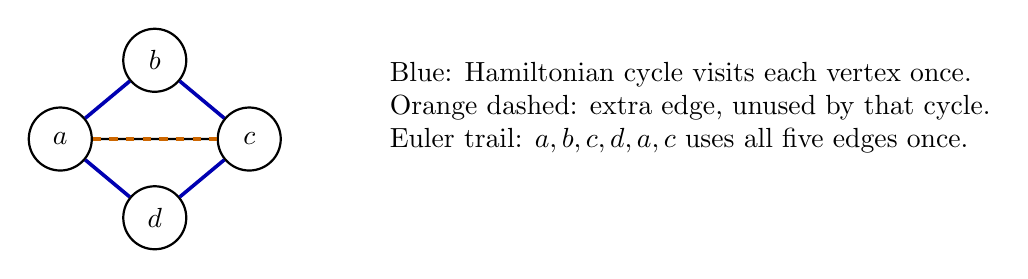
\begin{tikzpicture}[thick,every node/.style={circle,draw,fill=white,minimum size=8mm}]
\node (a) at (0,0) {$a$}; \node (b) at (1.2,1) {$b$}; \node (c) at (2.4,0) {$c$}; \node (d) at (1.2,-1) {$d$};
\draw (a)--(b)--(c)--(d)--(a) (a)--(c);
\draw[blue!70!black,line width=1.3pt] (a)--(b)--(c)--(d)--(a);
\draw[orange!80!black,line width=1.1pt,dashed] (a)--(c);
\node[draw=none,rectangle,align=left] at (8,0.4) {Blue: Hamiltonian cycle visits each vertex once.\\Orange dashed: extra edge, unused by that cycle.\\Euler trail: $a,b,c,d,a,c$ uses all five edges once.};
\end{tikzpicture}
\caption{Hamiltonian cycles cover vertices once; Euler trails cover edges once.}
\end{figure}

\Challenge{} The travelling salesperson problem asks for a minimum-weight Hamiltonian tour. Its optimisation version seeks the best tour; its decision version asks whether a tour of weight at most $B$ exists. No known algorithm solves all instances in time polynomial in the input size, but that is not a proof that no such algorithm exists.

\Challenge{} \textbf{Ore's theorem.} If $G$ has $n\geq 3$ vertices and every pair of nonadjacent vertices $u,v$ satisfies $\degG(u)+\degG(v)\geq n$, then $G$ has a Hamiltonian cycle.

\section*{Exercises}
\begin{enumerate}
\item Can a graph have exactly one odd-degree vertex? Why?
\item A connected graph has vertex degrees $2,2,4,4,2$. Does it have an Euler circuit? Explain.
\item Draw a connected graph with exactly two odd-degree vertices and give an Euler trail.
\item Give a connected graph where every vertex has degree at least 2 but no Hamiltonian cycle.
\item \Challenge{} Work through a proof of Ore's theorem. Suppose $u,v$ are nonadjacent and $\degG(u)+\degG(v)\geq n$. (a) If a Hamiltonian cycle in $G+uv$ avoids $uv$, explain why it is already in $G$; otherwise, delete $uv$ to obtain a Hamiltonian path $u=w_1,w_2,\ldots,w_n=v$ in $G$. (b) For $1\leq i\leq n-1$, let $I$ contain the indices for which $uw_{i+1}$ is an edge, and let $J$ contain those for which $w_iv$ is an edge. Explain why $|I|=\degG(u)$ and $|J|=\degG(v)$. (c) Since there are only $n-1$ indices, show that $I$ and $J$ overlap. Use an index in their intersection to rearrange the path edges into a Hamiltonian cycle in $G$. (d) Explain why adding such edges preserves the degree-sum condition for remaining nonadjacent pairs, and repeatedly add edges to deduce Ore's theorem.
\end{enumerate}
